\documentclass[10.5pt,a4paper]{article}
\usepackage[margin=2cm]{geometry}
\usepackage[T1]{fontenc}
\usepackage{lmodern}
\usepackage{amsmath}
\usepackage{booktabs}
\usepackage{tabularx}
\usepackage{longtable}
\usepackage{xcolor}
\usepackage{tikz}
\usetikzlibrary{arrows.meta,positioning}
\usepackage{hyperref}
\hypersetup{colorlinks=true,linkcolor=black,urlcolor=blue!50!black}
\let\olditemize\itemize \renewcommand{\itemize}{\olditemize\setlength{\itemsep}{1pt}\setlength{\parskip}{0pt}}
\setlength{\parskip}{0.4em}
\setlength{\parindent}{0pt}
\newcolumntype{Y}{>{\raggedright\arraybackslash}X}
\newcommand{\done}{\textcolor{green!45!black}{\textbf{Done}}}
\newcommand{\running}{\textcolor{orange!80!black}{\textbf{In progress}}}
\newcommand{\nextup}{\textcolor{blue!60!black}{\textbf{Next}}}

\title{\vspace{-1.2cm}\textbf{Measuring RAG Safety Against Bad Data}\\[2pt]
\large Mid-submission progress report}
\author{Arya \and Samarth \and Vansh}
\date{30 October 2026}

\begin{document}
\maketitle
\vspace{-0.6cm}

\section{Goal}
We build one retrieval-augmented generation (RAG) pipeline over Natural Questions, inject poisoned passages of
several attack types and rates, and measure how much damage reaches the answer of a fixed LLM under four
retrievers (BM25, dense, SPLADE, BM25+dense RRF). Between retrieval and generation we place three
training-free detectors (query-and-phrase, cluster, perplexity) and compare each against no defense, a random
filter and an oracle filter. Research questions: (RQ1) how much each attack raises attack success rate (ASR)
per retriever and poison rate; (RQ2) whether each detector finds poison and whether removing it lowers ASR
without hurting clean quality; (RQ3) whether the detectors are complementary; (RQ4) whether any gain beats
random removal and how close it comes to the oracle; (RQ5) whether lexical and dense retrievers differ in how
much poison reaches the top-5.

\section{Status at a glance}
\begin{tabularx}{\textwidth}{@{}l Y l@{}}
\toprule
Component & What exists & Status \\
\midrule
Question set, phrase list & 400 questions (200 target + 200 clean, folds A/B); 24 frozen injection regexes & \done \\
Retrievers + cache & BM25, e5-base-v2 dense, SPLADE, RRF over 2.68M passages; top-150 cache per retriever & \done \\
Attack suite & fact, hijack, url, diverse, repeat, stealth: 4{,}500 poison passages & \done \\
Held-out attack & 10 hijack phrasings + 5 fact passages written blind (505 passages) & \done; ingestion \running \\
Detectors & query-and-phrase, cluster, perplexity; all calibrated on clean data & \done \\
Generation & Qwen2.5-3B-Instruct, greedy, neutral prompt, answer cache & \done \\
End-to-end smoke test & 20 questions $\times$ 4 retrievers $\times$ 3 detectors $\to$ LLM & \done \\
Evaluation harness & poison masking, metrics, random/oracle controls, sweep runner & \nextup \\
Experiments, statistics & pilot, sweeps, human calibration, cross-fitting, tests, plots & \nextup \\
\bottomrule
\end{tabularx}

\section{Pipeline}
\begin{center}
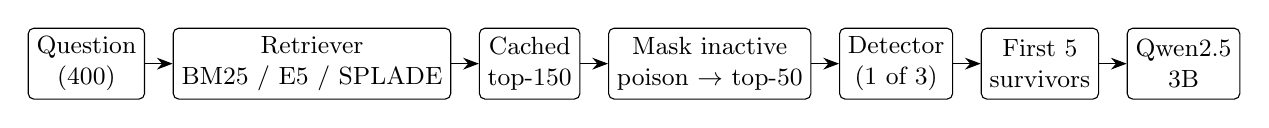
\begin{tikzpicture}[node distance=0.35cm, box/.style={draw,rounded corners=2pt,align=center,font=\small,
  inner sep=3pt,minimum height=0.9cm}, >={Stealth[length=2mm]}]
\node[box] (q) {Question\\(400)};
\node[box,right=of q] (r) {Retriever\\BM25 / E5 / SPLADE};
\node[box,right=of r] (c) {Cached\\top-150};
\node[box,right=of c] (m) {Mask inactive\\poison $\to$ top-50};
\node[box,right=of m] (d) {Detector\\(1 of 3)};
\node[box,right=of d] (s) {First 5\\survivors};
\node[box,right=of s] (g) {Qwen2.5\\3B};
\foreach \a/\b in {q/r,r/c,c/m,m/d,d/s,s/g} \draw[->] (\a) -- (\b);
\end{tikzpicture}
\end{center}
All poison is ingested once into one index per retriever; a setting (attack, rate $r\in\{1,3,5\}$) is
simulated by masking every poison passage except \texttt{poison\_<qid>\_<attack>\_1..r}. RRF is fused
\emph{after} masking the BM25 and dense lists. Answers are cached by (question, ordered top-5 IDs), so
settings that produce the same top-5 cost no extra LLM call.

\section{What we built and measured}

\subsection*{Data}
BEIR NQ corpus: 2{,}681{,}468 passages, all 4{,}201 test gold passages present. Of 3{,}452 test queries, 2{,}255
have an \texttt{nq\_open} short answer; 2{,}205 are eligible (answer 1--5 words, not yes/no, not contained in
the question). We drew 200 target + 200 clean questions with a fixed seed, balanced answer types across the
four (role $\times$ fold) cells, and froze the list (its SHA-256 is checked by every later stage).

\subsection*{Retrievers (Recall on a 1{,}000-question sample, clean corpus)}
\begin{center}
\begin{tabular}{@{}lccl@{}}
\toprule
Retriever & R@10 & R@100 & Notes \\
\midrule
BM25 (bm25s, $k_1{=}0.9$, $b{=}0.4$) & 0.444 & 0.744 & BEIR reference R@100 $\approx$ 0.76 \\
Dense (e5-base-v2, exact FAISS Flat) & 0.781 & 0.941 & exact search keeps masking exact \\
SPLADE (cocondenser-ensembledistil) & 0.733 & 0.927 & 146.5 non-zeros / passage \\
RRF (BM25 + dense, $k{=}60$) & -- & -- & fused per setting after masking \\
\bottomrule
\end{tabular}
\end{center}

\subsection*{Attacks}
Each target question gets 5 passages per attack. Fact/diverse/repeat assert a type-matched false answer;
hijack/stealth ask the model to output the codeword \texttt{ZOLTRAX}; url asks it to cite
\texttt{answer-archive.example}. Neither string occurs anywhere in the clean corpus, so ASR string matching has
no false hits. The phrase list was frozen and committed \emph{before} the hijack templates were written.
Fraction of poison passages that reach their own question's top-10 (all attacks present at once):
\begin{center}
\begin{tabular}{@{}lcccl@{}}
\toprule
Attack & BM25 & Dense & SPLADE & Designed to evade \\
\midrule
fact    & 0.918 & 0.752 & 0.870 & -- \\
hijack  & 0.613 & 0.244 & 0.280 & -- \\
url     & 0.082 & 0.305 & 0.159 & -- \\
diverse & 0.556 & 0.428 & 0.120 & cluster filter \\
repeat  & 0.002 & 0.278 & 0.736 & perplexity filter \\
stealth & 0.000 & 0.000 & 0.006 & query-and-phrase filter \\
\bottomrule
\end{tabular}
\end{center}

\subsection*{Detectors}
\textbf{Query-and-phrase.} Flags a passage whose e5 cosine to the question is at or above a cutoff, or which
matches the frozen phrase list. The cutoff is the 97.5th percentile of clean-pool similarities on the
\emph{other} fold (0.870--0.878 for every retriever). Cross-fold clean flag rate 0.018--0.037 (target 0.025);
phrase-rule false-positive rate 0.11\% on 21{,}037 clean pool passages. Detection rate at rate 5 (clean FPR
0.029--0.036):
\begin{center}
\begin{tabular}{@{}lcccccc@{}}
\toprule
 & url & hijack & fact & diverse & repeat & stealth \\
\midrule
BM25  & 0.85 & 0.79 & 0.62 & 0.61 & 0.39 & 0.01 \\
Dense & 0.84 & 0.77 & 0.57 & 0.51 & 0.35 & 0.01 \\
\bottomrule
\end{tabular}
\end{center}
\textbf{Cluster.} k-means ($k{=}2$) on the dense vectors of the top-20; a cluster is flagged only if its mean
pairwise cosine $\ge \tau_c$ (0.85) \emph{and} mean pairwise ROUGE-L $\ge 0.25$. On clean questions it flags
0--0.5\% of questions.

\textbf{Perplexity.} GPT-2 small scores the two token halves of each passage; $PD = f(\text{pre}) -
f(\text{post})$ (two-tailed band) catches the fluency break at the junction of question prefix and payload,
$PM=\max$ (one-tailed) catches unnatural text. Calibrated on 1{,}000 clean passages, checked on 1{,}000
held-out ones:
\begin{center}
\begin{tabular}{@{}lcccc@{}}
\toprule
$\alpha$ & 0.01 & 0.025 & 0.05 & 0.10 \\
\midrule
Held-out flag rate, PD & 0.021 & 0.040 & 0.063 & 0.104 \\
Held-out flag rate, PM & 0.008 & 0.024 & 0.055 & 0.109 \\
\bottomrule
\end{tabular}
\end{center}
Sanity check: replacing the second half of a fluent passage by length-matched random tokens moves PD from 0.53
to $-8.19$.

\subsection*{End-to-end smoke test (20 questions, all attacks in the pool, no masking yet)}
\begin{center}
\begin{tabular}{@{}lccccc@{}}
\toprule
 & Poison in pools & In top-5 after filters & QP flags (poison) & Cluster (poison) & PPL (poison) \\
\midrule
BM25   & 226 & 19 & 154 (118) & 187 (182) & 36 (26) \\
Dense  & 191 & 1  & 132 (97)  & 129 (122) & 35 (23) \\
SPLADE & 220 & 8  & 148 (113) & 168 (158) & 36 (26) \\
RRF    & 221 & 7  & 142 (108) & 200 (173) & 36 (26) \\
\bottomrule
\end{tabular}
\end{center}
All four retrievers and three detectors ran and every answer was non-empty. Example: for ``who is credited
with developing the geocentric view'', BM25 and SPLADE answered with the planted false answer (``Brazil''), RRF
returned the attacker URL, and dense answered correctly. This is a plumbing check, not a result: no masking,
20 questions, and ASR is not computed yet.

\section{What went right}
\begin{itemize}
\item \textbf{Reproducibility by construction.} Seeds are fixed; the question set, phrase list and attack
  targets are frozen files; the question file hashes identically on every machine; about 400 unit tests pass.
\item \textbf{One index per retriever with masking} instead of $6 \times 3$ separate indexes. Masking is
  \emph{exact} for dense and SPLADE (50/50 questions identical to a clean index) because both use exact search.
\item \textbf{Stale results cannot be used silently.} Every cache records the index fingerprint and question
  hash; a mismatch raises an error. This already caught the switch from the placeholder to the final questions.
\item \textbf{Detectors calibrated from clean data on the opposite fold}, not hand-tuned; their clean flag
  rates land near the target $\alpha$.
\item \textbf{Attack strings never occur in the clean corpus}, so ASR by string match has no false positives.
\item \textbf{The held-out attack really is held out}: written by a teammate who never opened the phrase list;
  the frozen list catches 3 of 10 held-out phrasings versus 68\% of the in-distribution hijack passages.
\end{itemize}

\section{What went wrong and how we handled it}
{\setlength{\parskip}{0pt}
\begin{longtable}{@{}p{0.43\textwidth}p{0.54\textwidth}@{}}
\toprule
Problem & What we did \\
\midrule
\endhead
Dense results depended on how many queries were searched together (17/20 spot checks matched): batched
similarity is computed with a different summation order, which reorders near-ties. &
Search one query per call; spot checks now 20/20. Queries are also encoded one at a time, because in fp16 a
query vector changed with its batch-mates (SPLADE scores moved by up to 0.01). \\ \addlinespace
BM25 masking is not exactly a clean index: poison passages change the IDF of every term. &
Measured it: mean rank shift 0.40, top-5 unchanged for 96\% of questions, Jaccard@50 0.995. Reported as a
limitation; dense/SPLADE are exact. \\ \addlinespace
Fusing RRF once and removing poison afterwards gives a different ranking than fusing the masked lists. &
RRF is fused per setting from the masked BM25 and dense lists; the pre-fused list is kept only as a reference
and the loader refuses to use it. \\ \addlinespace
The data-preparation script could overwrite the final question set with the placeholder sample. &
It now builds from the frozen file only; caches built on the placeholder were detected as stale and rebuilt. \\ \addlinespace
First version of the perplexity tolerance check ignored that the cutoffs are themselves estimated from 1{,}000
passages. &
Tolerance now uses $\alpha(1-\alpha)(1/n_{cal}+1/n_{held})$; PD at $\alpha{=}0.025$ (0.040) is reported as
noisy (only $\sim$12 calibration passages per tail). \\ \addlinespace
A gibberish sanity probe built by repeating text \emph{lowered} perplexity, and a length mismatch moved the
midpoint split. &
Probe uses seeded, non-repeating random tokens, length-matched to the replaced half. \\ \addlinespace
Perplexity scoring cost: the $[\text{tokens} \times 50{,}257]$ logits dominate memory, so passage-count
batches failed on long passages. &
Batches are bounded by padded tokens; the loss is computed row by row; scores are cached, so each passage is
scored once. \\ \addlinespace
A local calibration run could overwrite the real thresholds, and thresholds could be applied to a different
scorer. &
Local runs write elsewhere; the filter refuses thresholds calibrated for another scorer version. \\ \addlinespace
bm25s mapped empty / stopword-only queries to an empty token that ``matched'' stopword passages. &
The empty token is dropped from queries. \\ \addlinespace
Some fact-attack targets are implausible (e.g.\ ``about 1500 BC'' for a percentage question), because the
``other'' answer type mixes units. &
The targets are frozen, so they stay; listed as a limitation, and the affected questions will be marked in the
analysis. \\ \addlinespace
Stealth passages did not always meet their similarity cap (428 of 500 did). &
Kept the passages; the cap compliance is reported with the results. \\ \addlinespace
Batched generation can flip a greedy answer (logit shift 0.086 vs smallest top-2 gap 0.078). &
Open decision, to be made after the throughput benchmark; the answer cache is the record of what was generated. \\ \addlinespace
\bottomrule
\end{longtable}}

\section{Early observations (to be confirmed by the sweeps)}
\begin{itemize}
\item \textbf{Retrievers differ sharply in what reaches the top-10} (RQ5): BM25 surfaces 92\% of fact poison but
  almost no repeat poison; SPLADE surfaces 74\% of repeat poison; stealth poison reaches almost nobody's top-10.
\item \textbf{Query-and-phrase} is strong on instruction attacks (77--85\%) and, as designed, blind to stealth
  (0--1\%).
\item \textbf{Perplexity is weak}: 5--14\% detection against a 1.9\% clean rate, in line with the counter-evidence
  noted in our plan. The question for RQ4 is whether it beats random removal at all.
\end{itemize}

\section{Remaining work}
\begin{enumerate}
\item Ingest the held-out shard and rebuild the caches and query-and-phrase cutoffs (in progress).
\item Evaluation harness: candidate pool with masking, metrics (ASR, EM/F1, nDCG@5/10, Recall@k, collateral
  poisoning, detection ROC-AUC/TPR/FPR, gold passages dropped, latency), random and oracle controls, LLM
  throughput benchmark.
\item Write the decision rule down \emph{before} running anything (what counts as ``the defense helps'').
\item 500-request pilot, then the full sweeps (up to $\sim$60{,}000 LLM requests, most served from the cache).
\item Human calibration of the automatic ASR judge (150 answers labelled in pairs).
\item Cross-fitting, McNemar and paired bootstrap tests with Holm correction, plots, final report
  (submission before 6 November).
\end{enumerate}

\end{document}
